%%%%%%%%%%%%%%%%%%%%%%%%%%%%%%%%%%%%%%%%%%%%%%%%%%%%%%%%%%%%%%%%%%%%%%%%%%%%%%%%
% SD Lab -- Async Programming
% Giovanni Ciatto
% Alma Mater Studiorum - Università di Bologna
% mailto:giovanni.ciatto@unibo.it
%%%%%%%%%%%%%%%%%%%%%%%%%%%%%%%%%%%%%%%%%%%%%%%%%%%%%%%%%%%%%%%%%%%%%%%%%%%%%%%%
%\documentclass[handout]{beamer}\mode<handout>{\usetheme{default}}
%
\documentclass[presentation]{beamer}\mode<presentation>{\usetheme{AMSBolognaFC}}
%\documentclass[handout]{beamer}\mode<handout>{\usetheme{AMSBolognaFC}}
%%%%%%%%%%%%%%%%%%%%%%%%%%%%%%%%%%%%%%%%%%%%%%%%%%%%%%%%%%%%%%%%%%%%%%%%%%%%%%%%
\usepackage{sd-lab-common}
\usepackage{sd-lab-async-programming}
%%%%%%%%%%%%%%%%%%%%%%%%%%%%%%%%%%%%%%%%%%%%%%%%%%%%%%%%%%%%%%%%%%%%%%%%%%%%%%%%
\title[\currentLab{} -- Async 101]{
	Asynchronous Programming 101
}
%
\subtitle{\courseName{} (\courseAcronym) / Module \moduleN{}}
%
\author[\sspeaker{\gcShort} \& \mmShort]{
	\speaker{\gcFull} \and \mmFull
	\\ 
	\gcEmail \and \mmEmail
}
%
\institute[\disiShort, \uniboShort]{\disi{} (\disiShort)\\\unibo}
%
\date[A.Y. \academicYear{}]{Academic Year \academicYear{}}
%
\begin{document}

%\\\\\\\\\\\\\\\\\\\\\
\frame{\titlepage}
%\\\\\\\\\\\\\\\\\\\\\

\section{Overview}

\begin{frame}[c]{Motivation \& Lecture Goals}

\begin{itemize}
	\item asynchronous programming is a fundamental paradigm for distributed or concurrent systems

	\vfill

	\item in particular in this course we need it to program mechanisms for distributed interaction

	\vfill

	\item furthermore, asynchronous programming is the \emph{de facto} standard for the development of real-world distributed applications

	\vfill

	\item for all those reasons, in this tutorial we introduce the notions of \alert{executor service}, \alert{future}, and \alert{promise} in Java
	%
	\begin{itemize}
		\item equivalent constructs exist in all mainstream languages nowadays
	\end{itemize}
\end{itemize}

\end{frame}

\begin{frame}[c]{Lab \labN{} Repository on GitLab}

	\begin{itemize}
		\item examples and exercises described in this lecture are provided by means of the following GitLab repository:
		%
		\begin{center}
			\uurl{\labRepo}
		\end{center}

		\vfill

		\item clone it on your machine using Git
		%
		\begin{itemize}
		    \item[\$] \texttt{git clone \textit{<repo URL>}}
		\end{itemize}

		\vfill

		\item even if a minimal environment simply relying on a text editor + Gradle is sufficient for this lab, we kindly suggest to import the cloned repository into some IDE, e.g. IntelliJ Idea or Eclipse

		\vfill

		\item in order to be able to submit your exercises, please ensure you requested access to the \href{\gitlabGroup}{GitLab group of the course}
	\end{itemize}

\end{frame}

\section{Fundamentals}

\subsection{Operative Systems Recap}

\begin{frame}[allowframebreaks]
    \frametitle{OS, Processes, Threads, etc.}

    \begin{block}{Operative System (OS)}
        The entity mediating or virtualising the access of users' applications to:
        %
        \begin{itemize}
            \item the processor(s)
            \item the (RAM) memory
            \item the file system
            \item I/O peripherals
        \end{itemize}
        i.e. any hardware resource composing a machine
        %
        \begin{itemize}
            \item[$\rightarrow$] virtualisation is needed to support
            %
            \begin{itemize}
                \item isolation
                \item hardware / driver agnosticism
            \end{itemize}
            \item[$\rightarrow$] mediation is needed to shared access
        \end{itemize}
    \end{block}

    \begin{block}{Scheduling}
        The functionality letting an OS execute $N$ activities on $M$ processors
        %
        \begin{itemize}
            \item even if $N \gg M$
            \item even if $M \equiv 1$
        \end{itemize}
    \end{block}

    \begin{block}{Virtual Memory}
        The functionality letting each activity running within the OS
        %
        \begin{itemize}
            \item have its own isolated memory (address space)
            \item pretending to be the only one
            \item avoid to pollute other activities' memory
        \end{itemize}
    \end{block}

    \begin{block}{Process vs. Thread}
        The two main sorts of activities which can run within an OS
        %
        \begin{description}
            \item[processes] are independent running programs, within the same OS
            %
            \begin{itemize}
                \item each one has its own address space
                %
                \begin{itemize}
                    \item[$\rightarrow$] no memory contamination is possible
                    \item[$\rightarrow$] interaction among processes can occur via I/O and pipes
                \end{itemize}
            \end{itemize}

            \item[threads] are independents control flows running within a process
            %
            \begin{itemize}
                \item all threads can access the same process memory
                %
                \begin{itemize}
                    \item[$\rightarrow$] interaction among threads may occur via shared memory
                \end{itemize}
            \end{itemize}
        \end{description}
    \end{block}

    \begin{block}{I/O and Files}
        Three main abstractions:
        %
        \begin{description}
            \item[files] --- letting processes interact with each others or the HW
            %
            \begin{itemize}
                \item[ie] \alert{streams} of data which can be byte-wise \alert{read/written}
                %
                \begin{itemize}
                    \item via a \alert{blocking} API for reading/writing
                \end{itemize}
            \end{itemize}

            \item[file system] --- a \alert{tree}-like way of organising and \alert{referencing}/naming files

            \item[path] --- the particular name of a file in a file system
        \end{description}
    \end{block}
\end{frame}

\begin{frame}[allowframebreaks]
    \frametitle{Parallel vs. Concurrent}

    \begin{block}{Single-Core vs. Multi-Core Processors}
        \begin{itemize}
            \item 1-core machines can normally perform a \alert{single operation} at a time
            \item $N$-core machines can typically perform \alert{$N$ simultaneous operations}
            %
            \begin{itemize}
                \item yet, a single memory access at a time
                \item fundamental role of \alert{cores' caches} to speedup computations
            \end{itemize}
        \end{itemize}
    \end{block}

    \begin{alertblock}{Takeways}
        \centering
        Thanks to scheduling, concurrency can exist on single-core machines too!
    \end{alertblock}

    \begin{block}{Concurrent $\supset$ Parallel}
        \begin{description}
            \item[parallel] activities are actually simultaneous
            %
            \begin{itemize}
                \item as they are executed by different processors / cores
            \end{itemize}

            \item[concurrent] activities may or may not be simultaneous
            %
            \begin{itemize}
                \item[eg] a queue of tasks being executed by $N$ distributed processors
                %
                \begin{itemize}
                    \item they are concurrent, yet not parallel
                \end{itemize}
            \end{itemize}
        \end{description}
    \end{block}
\end{frame}

\subsection{Understanding Concurrency}

\begin{frame}[allowframebreaks]
    \frametitle{Control Flow}

    \begin{block}{Rough definition(s)}
        \begin{center}
            The order in which a program statements are executed
        \end{center}
    \end{block}

    \begin{block}{Synchronus statements}
        \begin{itemize}
            \item In sequential programs, statements are executed \alert{synchronously}
            %
            \begin{itemize}
                \item[ie] one after another
                \item[ie] statement $i+1$ is only executed after statement $i$ is over
                %
                \begin{itemize}
                    \item[$\rightarrow$] the ``end'' of statements is implicitly defined
                \end{itemize}
            \end{itemize}
        \end{itemize}
    \end{block}

%    \tcodeview{2}{7}{30}{\tiny}{\codepath{Misc/Program.cs}}{Sequential Control Flow}
    \lstinputlisting[basicstyle=\tiny\ttfamily, language=Java, caption={Sequential Control Flow}]{code/SequentialControlFlow.java}

    % Ordinary notion of control flow

    % Notion of synchronous operation

    % Operations'ending is implicitly developed

    \begin{alertblock}{Takeway}
        \begin{itemize}
            \item Concurrency is about \alert{coordinating} multiple interacting activites
            %
            \begin{itemize}
                \item each one having its own control flow
            \end{itemize}
        \end{itemize}
    \end{alertblock}

    \begin{exampleblock}{Control flows in practice}
        \begin{itemize}
            \item In this section: 1 control flow $\approx$ 1 thread
            \item In general this is not true!
            %
            \begin{itemize}
                \item via \alert{asynchronous programming}, $N$ control flows may run on 1 thread
            \end{itemize}
        \end{itemize}
    \end{exampleblock}
\end{frame}

\subsubsection{Multi-threading}

\begin{frame}
    \frametitle{Why Multi-threading}

    \begin{alertblock}{Discalimer}
        \begin{itemize}
            \item \alert{Threads} and \alert{multi-threading}  are the basic bricks of concurrency

            \item However, far wiser approaches exist to concurrency
            %
            \begin{itemize}
                \item \alert{asynchronous programming} is one of them
            \end{itemize}
        \end{itemize}
    \end{alertblock}

\end{frame}

\begin{frame}[allowframebreaks]
    \frametitle{Multiple Concurrent Threads}

    \begin{block}{Threads}
        \begin{itemize}
            \item Threads are control flows, managed and scheduled by the OS
            \item They run inside the same process and can share its memory
            \item Each thread has its own call stack \& program counter
            %
            \begin{itemize}
                \item multiple threads execution is actually independent
                %
                \begin{itemize}
                    \item as long as they don't access a common portion of memory
                \end{itemize}
            \end{itemize}
        \end{itemize}
    \end{block}

    \begin{exampleblock}{Common operations over threads}
        \begin{description}
            \item[creation] --- lets a thread create another thread from a \alert{procedure}
            %
            \begin{itemize}
                \item creation usually does not imply start
                \item the procedure represents an action to be performed
                %
                \begin{itemize}
                    \item by the new thread, upon start
                \end{itemize}
            \end{itemize}

            \item[start] (a.k.a. fork, spawn) --- lets a thread spawn another thread
            %
            \begin{itemize}
                \item threads can usually be started only once
            \end{itemize}

            \item[join] (a.k.a. wait, await) --- lets a thread wait for another thread termination
            %
            \begin{itemize}
                \item only started threads can be joined
            \end{itemize}
        \end{description}
    \end{exampleblock}

    \begin{center}
        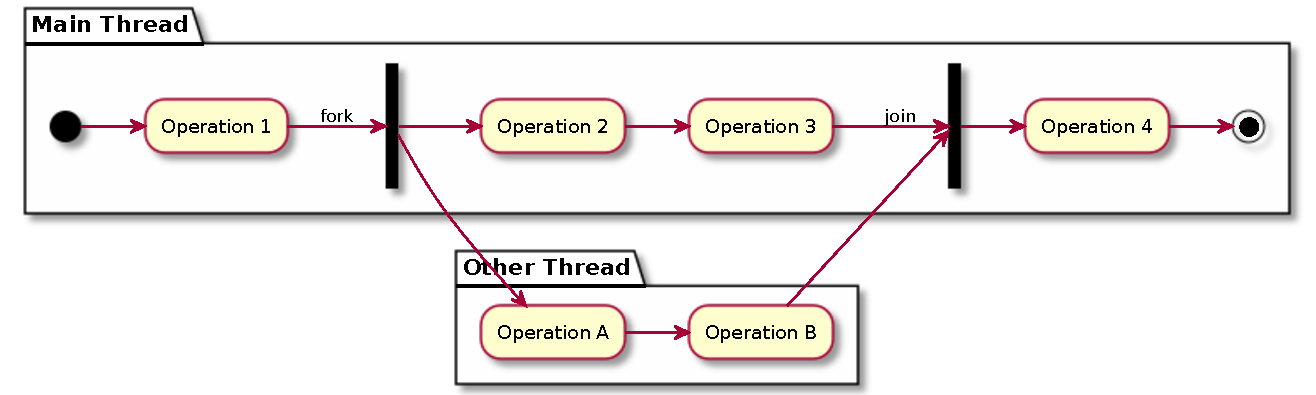
\includegraphics[width=\linewidth]{img/fork-join.pdf}
    \end{center}
    %
    \begin{itemize}
        \item \texttt{Operation 1} is certainly executed first
        \item \texttt{Operation 4} is certainly executed last
        \item \texttt{Operation 2} is certainly executed before \texttt{Operation 3}
        \item \texttt{Operation A} is certainly executed before \texttt{Operation B}
        \item nothing else is certain!
    \end{itemize}

    \framebreak

    \begin{block}{Threads on the JVM}
        \begin{itemize}
            \item Each JVM application is executed on a main thread
            %
            \begin{itemize}
                \item the garbage collector is usually executed on yet another thread
            \end{itemize}

            \item Novel threads may be created/started/joined
            %
            \begin{itemize}
                \item threads are instances of the \texttt{java.lang.\alert{Thread}} class
                %
                \begin{itemize}
                    \item notice that threads are modelled as objects in the JDK
                \end{itemize}
            \end{itemize}

            \item Our code is always executed on some thread
            %
            \begin{itemize}
                \item be it the main thread or anther thread we created after it
            \end{itemize}
        \end{itemize}
    \end{block}

    \begin{exampleblock}{Useful functionalities of \texttt{java.lang.Thread}}
        \begin{description}
            \item[\texttt{new Thread(Runnable)}] --- creates a novel thread which shall execute the provided \texttt{Runnable} upon start

            \item[\texttt{start()}] lets another thread start the thread

            \item[\texttt{join()}] lets another thread wait for a thread termination

            \item[\texttt{interrupt()}] lets a thread resume another \alert{blocked} thread
            %
            \begin{itemize}
                \item[!] this does not terminate the latter thread!
            \end{itemize}

            \item[\texttt{stop()}] lets a thread terminate another thread
            %
            \begin{itemize}
                \item[!] avoid terminating threads from the outside
                %
                \begin{itemize}
                    \item[$\rightarrow$] threads should be responsible for their own termination
                \end{itemize}
            \end{itemize}
        \end{description}
    \end{exampleblock}

    \framebreak

%    \codeview{1}{5}{28}{\tiny}{\codepath{Thread1/Program.cs}}
    \lstinputlisting[basicstyle=\tiny\ttfamily, language=Java]{code/Thread1.java}

    \framebreak

    \begin{alertblock}{Asynchrnous activities}
        \begin{itemize}
            \item Notice that the execution of \texttt{threadMain()} is \alert{asynchronous}
            %
            \begin{itemize}
                \item in the eyes of the main thread
            \end{itemize}

            \item The main thread knows when it starts, not when it ends
            %
            \begin{itemize}
                \item unless the second thread is join
            \end{itemize}
        \end{itemize}
    \end{alertblock}
\end{frame}

\begin{frame}[allowframebreaks]
    \frametitle{Consequences of Concurrency}

    \begin{block}{Non-determinism}
        \begin{itemize}
            \item The way the OS will schedule concurrent threads is unpredictable
            \item Different runs of a concurrent program may produce different outcomes
            %
            \begin{itemize}
                \item because execution may proceed differently in different runs
            \end{itemize}
            \item[$\rightarrow$] Non-deterministic observable behaviour of the system
        \end{itemize}
    \end{block}

    \begin{block}{Interleaving}
        \begin{itemize}
            \item \alert{Atomic} actions of concurrent threads may unpredictably \alert{interleave}
            \item All possible total ordering among atomic actions may occur
            %
            \begin{itemize}
                \item in principle
                \item despite with different probabilities
            \end{itemize}
            \item Unpredictability of interleaving $\rightarrow$ Non-determinism
        \end{itemize}
    \end{block}

    \framebreak

    \begin{center}
        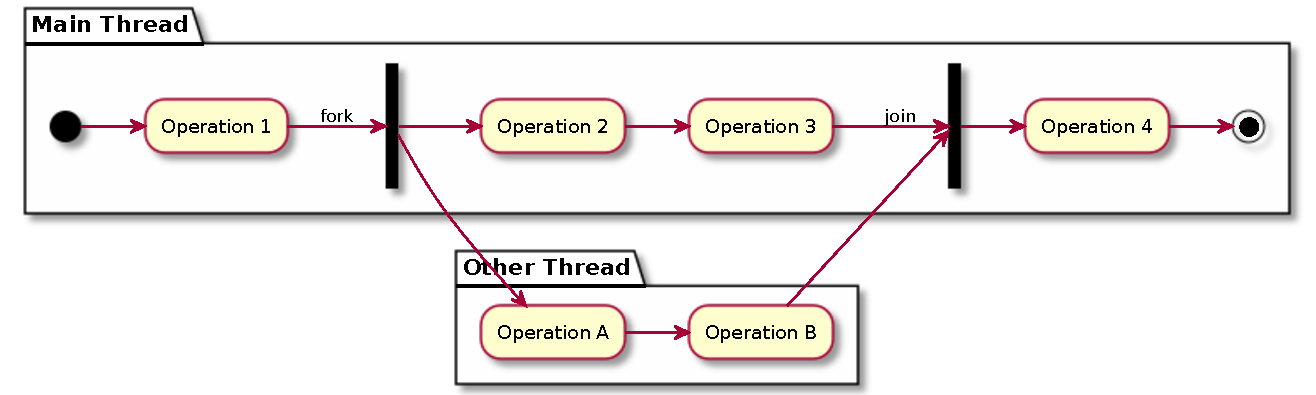
\includegraphics[width=\linewidth]{img/fork-join.pdf}
    \end{center}

    \begin{exampleblock}{Possible interleavings}
        \begin{multicols}{3}
            \begin{itemize}
                \item 1, 2, 3, A, B, 4
                \item 1, 2, A, 3, B, 4
                \item 1, 2, A, B, 3, 4
                \item 1, A, 2, B, 3, 4
                \item 1, A, B, 2, 3, 4
            \end{itemize}
        \end{multicols}
    \end{exampleblock}

%    \framebreak

%    \codeview{1}{7}{32}{\tiny}{\codepath{Thread1/Program.cs}}
%    \lstinputlisting[basicstyle=\tiny\ttfamily]{code/Thread1.txt}

\end{frame}

\begin{frame}[allowframebreaks]
    \frametitle{Advanced Aspects of Threads}

    % Synchronization (Suspend/Block -- Resume/Release)

    % Join/Wait/Await

    \begin{exampleblock}{More functionalities of threads}
        \begin{description}
            \item[suspend] (a.k.a. block, wait)  --- lets a thread pause its own execution

            \item[resume] (a.k.a. release) --- lets a thread resume another thread
            %
            \begin{itemize}
                \item assumes the latter thread has been previously suspended
            \end{itemize}

            \item[synchronization] (a.k.a. barrier) --- lets 2 threads wait for each other to reach a particula point in their execution
            %
            \begin{itemize}
                \item implies both threads suspending and resuming
            \end{itemize}
        \end{description}
    \end{exampleblock}

    \begin{alertblock}{Important notice about the JVM}
        \begin{itemize}
            \item Despite methods exist to suspend/resume instanced of \texttt{Thread}\ldots
            %
            \begin{itemize}
                \item[eg] \texttt{resume()}, \texttt{suspend()}
                \item \ldots \textbf{do not use them!}
            \end{itemize}

            \item Suspend/resume should only be performed via adequate mechanisms
            %
            \begin{itemize}
                \item[eg] monitors, or semaphores
            \end{itemize}

            \item Also notice that the following operations involve suspension/resume:
            %
            \begin{description}\small
                \item[\texttt{Thread.sleep(\cscat{Millis})}] --- suspends the current thread for a while
                \item[\texttt{join()}] --- lets a thread await for another thread termination
                \item[I/O facilities] --- for reading or writing over streams
                %
                \begin{itemize}
                    \item imply potential blocking/resuming
                    %
                    \begin{itemize}
                        \item to guarantee a synchronous semantics
                    \end{itemize}

                    \item[eg] \texttt{System.in.\textit{read*}()} or \texttt{System.out.\textit{print*}(\ldots)}
                \end{itemize}
            \end{description}
        \end{itemize}
    \end{alertblock}

    \framebreak

    \begin{figure}
        \centering
        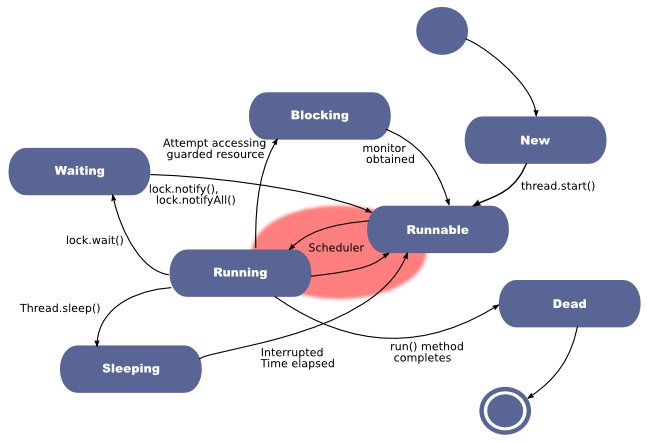
\includegraphics[width=.7\linewidth]{img/thread-states.png}
        \caption{Admissible states of a JVM thread}
    \end{figure}

\end{frame}

\begin{frame}[allowframebreaks]
    \frametitle{Threads and I/O}

    \begin{alertblock}{Takeway}
        \begin{itemize}
            \item I/O stream reading/writing operations are \alert{blocking}
            %
            \begin{itemize}
                \item you may not notice that if the operation is \alert{local}
            \end{itemize}
        \end{itemize}
    \end{alertblock}

    \framebreak

    \startDemo
    \begin{exampleblock}{Demo \currentDemo{} -- One thread reading multiple files}
        \begin{itemize}
            \item Consider the \texttt{sd.lab.concurrency.\alert{MultiReadingThread}*} classes
            \item it's a single thread reading multiple files in a \alert{round-robin} fashion:
            %
            \begin{description}\small
                \item[\texttt{file1.txt}] containing lines \texttt{a}, \texttt{b}, \texttt{c}
                \item[\texttt{file2.txt}] containing lines \texttt{1}, \texttt{2}, \texttt{3}
                \item[\texttt{file3.txt}] containing lines $\mathtt{\alpha}$, $\mathtt{\beta}$, $\mathtt{\gamma}$
                \item[standard input] containing any line you may write 
            \end{description}
            \item If the standard input is included among the files to be read:
            %
            \begin{itemize}
                \item the execution of the thread will block until you write some line
                \item any other activity is stuck until then
            \end{itemize}
            \item Total ordering of reads is \alert{predictable}
        \end{itemize}
    \end{exampleblock}

    \framebreak

    \startDemo
    \begin{exampleblock}{Demo \currentDemo{} -- Multiple threads reading multiple files}
        \begin{itemize}
            \item Consider the \texttt{sd.lab.concurrency.\alert{MultiReadingService}*} classes
            \item it's a program reading multiple files, using \alert{one thread per file}:
            %
            \begin{itemize}
                \item same files as above
            \end{itemize}
            \item If one thread is blocked, the others can progress anyway
            \item Total ordering of reads is \alert{unpredictable}
            %
            \begin{itemize}
                \item per-file ordering of reads is predictable, instead
            \end{itemize}
        \end{itemize}
    \end{exampleblock}

    \framebreak

    \begin{block}{How do we test concurrent systems?}
        \begin{itemize}
            \item Consider classes \texttt{sd.lab.concurrency.\alert{TestMultiReading}*}
            %
            \begin{itemize}
                \item and the test units therein defined (i.e. methods annotated with \texttt{@Test})
            \end{itemize}
            \item All such unit tests follow a similar pattern:
            %
            \begin{enumerate}
                \item initialize some collection $C$ 
                \item configure the system to push all relevant \alert{observable} events in $C$
                \item start the system
                \item wait for the system to terminate
                \item draw assertions about \alert{which} event occurred
                %
                \begin{itemize}
                    \item possibly, draw assertions about the (partial) \alert{ordering} of events
                \end{itemize}
            \end{enumerate}
        \end{itemize}
    \end{block}

\end{frame}

\begin{frame}[allowframebreaks]
    \frametitle{State graph of a concurrent system}

    \begin{block}{Definition}
        \begin{itemize}
            \item A directed graph where
            %
            \begin{description}
                \item[nodes] represent admissible \alert{global} states of the system
                %
                \begin{itemize}
                    \item i.e. assignments of \alert{all} variables of the systems
                    \item including all program counters of all threads
                    \item including all fields of all objects used by all threads
                \end{itemize}

                \item[edges] represent admissible state transition
                %
                \begin{itemize}
                    \item due to any thread executing a single atomic operation
                    \item each node has an outgoing edge for each possible state transition
                \end{itemize}
            \end{description}
        \end{itemize}
    \end{block}

    \framebreak

%    \tcodeview{1}{6}{27}{\tiny}{\codepath{Thread2/Program.cs}}{Example of concurrent system\dots}
    \lstinputlisting[basicstyle=\tiny\ttfamily, language=Java, caption={Example of concurrent system\dots}]{code/Thread2.java}

    \framebreak

    \begin{center}
        \ldots and its state graph ($> 18$ states!)

        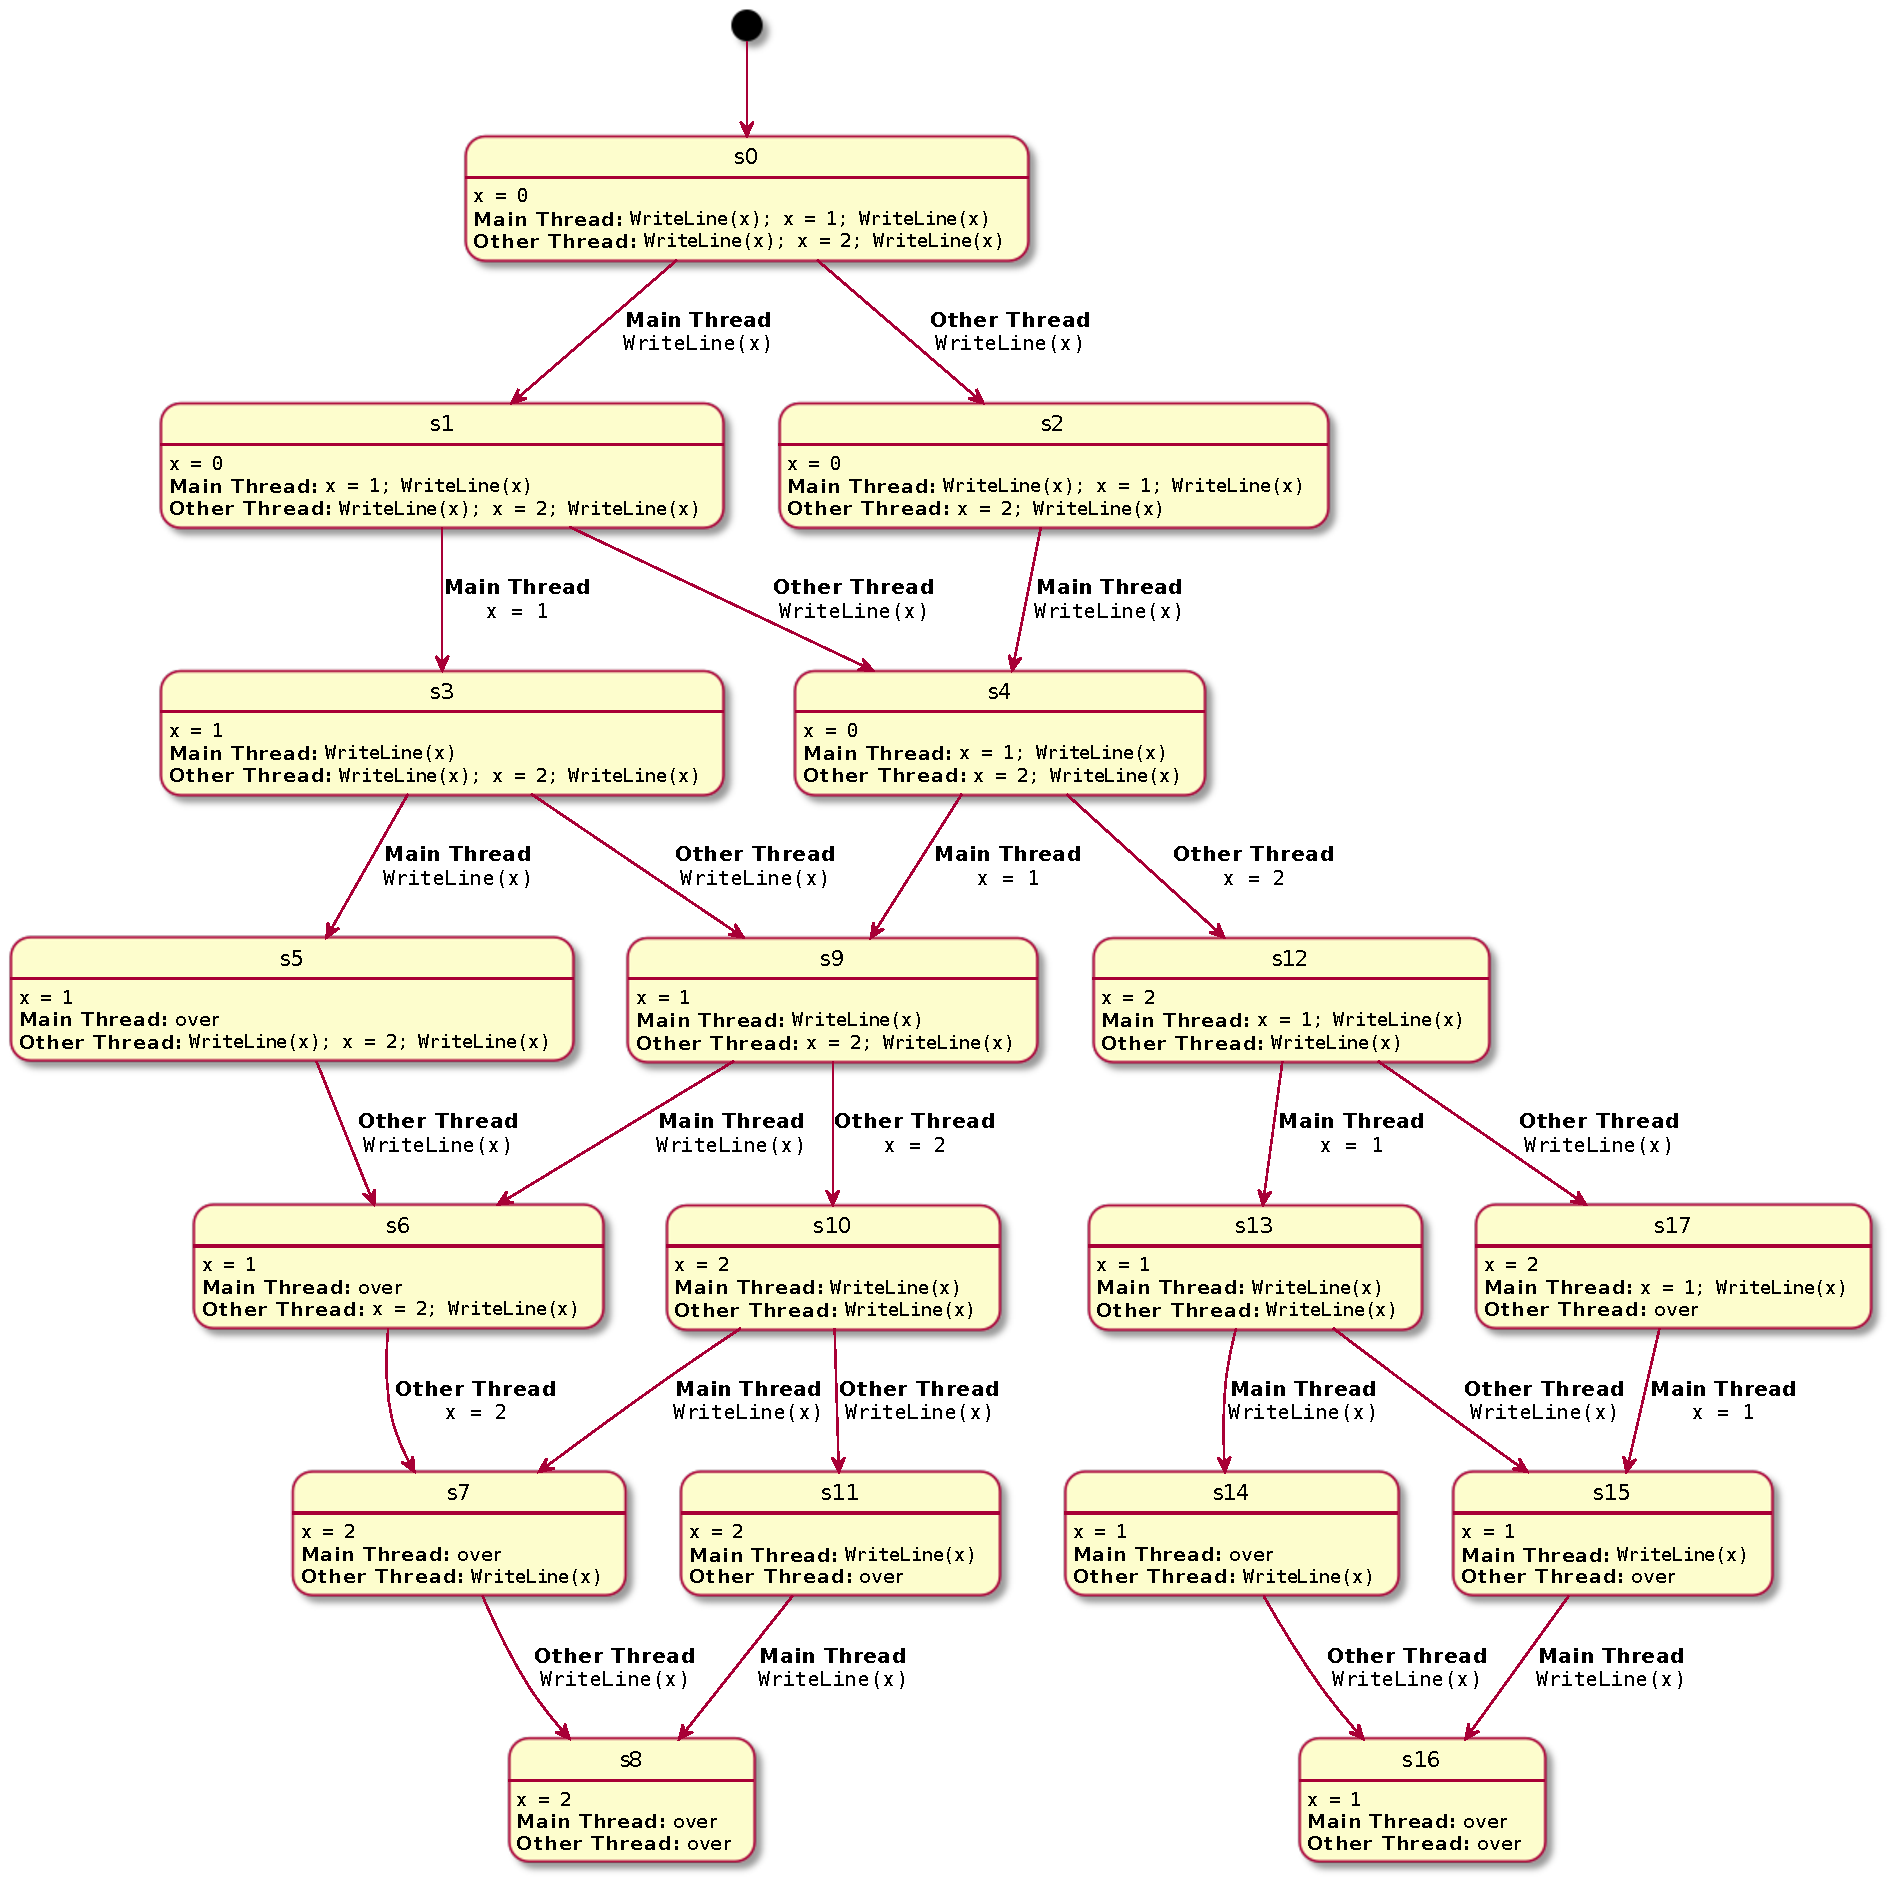
\includegraphics[height=.7\textheight]{img/state-diagram.pdf}
    \end{center}

    \framebreak

    \begin{alertblock}{Recall that}
        \begin{itemize}
            \item When you launch a concurrent system, you can observe a single run
            %
            \begin{itemize}
                \item among the many possible ones
            \end{itemize}

            \item This corresponds to one particular path in the state graph
            %
            \begin{itemize}
                \item from the initial state to some ending state
                %
                \begin{itemize}
                    \item \ldots assuming that an ending state even exist
                \end{itemize}
            \end{itemize}
        \end{itemize}
    \end{alertblock}

\end{frame}

\section{Asynchronous Programming}

\subsection{Executor Services}

\begin{frame}[c,allowframebreaks]{Executor Services}

	\begin{itemize}
		\item objects of type \href{https://docs.oracle.com/javase/8/docs/api/java/util/concurrent/ExecutorService.html}{\texttt{java.util.concurrent.\alert{ExecutorService}}} are useful for building \alert{concurrent} applications, abstracting threads away

		\bigskip

		\item an \alert{\texttt{ExecutorService}} is essentially a wrapper for one or more \alert{worker} threads + a \alert{task queue} which is consumed by such thread(s), where a task can be either:
		%
		\begin{itemize}
			\item an instance of \href{https://docs.oracle.com/javase/8/docs/api/java/lang/Runnable.html}{\texttt{java.lang.\alert{Runnable}}}, representing a \emph{procedure} to be \alert{executed} by the executor service

			\item an instances of \href{https://docs.oracle.com/javase/8/docs/api/java/util/concurrent/Callable.html}{\texttt{java.util.concurrent.\alert{Callable<X>}}}, representing a \emph{function}, returning type \texttt{X}, to be \alert{submitted} to the executor service
		\end{itemize}

		\bigskip

		\item Executor Services can be created by means of the \href{https://docs.oracle.com/javase/8/docs/api/java/util/concurrent/Executors.html}{\texttt{java.util.concurrent.Executor\alert{s}.new*()}} static methods
	\end{itemize}

	\framebreak

	\begin{center}
		\includegraphics[width=.9\linewidth]{img/executor_service.jpg}

		{\tiny Source: \url{https://www.callicoder.com/java-executor-service-and-thread-pool-tutorial/}}
	\end{center}

	\framebreak

	\lstinputlisting[language=Java]{code/ExecutorService.java}

\end{frame}

\subsection{Runnables}

\begin{frame}[c,allowframebreaks]{Executing \texttt{Runnable}s -- Concept}

	\lstinputlisting[language=Java]{code/Runnable.java}

	\framebreak

	\begin{itemize}
		\item runnables can be \alert{executed} on an executor service by means of its \texttt{void execute(Runnable task)} method
	\end{itemize}
	%
	\begin{center}
		\includegraphics[width=.7\linewidth]{img/execute.pdf}
	\end{center}
	%
	\hint{When the \texttt{execute()} method returns, there is \alert{no guarantee} the task has \alert{already} been executed}

\end{frame}

\begin{frame}[c]{Executing \texttt{Runnable}s -- Example}

	\lstinputlisting[language=Java]{./code/execute_example.java}

	\vfill

	\begin{itemize}
		\item \texttt{void shutdown()} prevents the executor service from accepting other tasks
	\end{itemize}

\end{frame}

\begin{frame}[c]{More examples on \texttt{ExecutorService}s}

	Let's have a look to \texttt{sd.lab.concurrency.\alert{ExecutorServicesExamples}}

	\vfill

	\begin{block}{How to run a specific test in Gradle}
		\begin{itemize}
			\item[\$] \texttt{./gradlew cleanTest test --tests "full.package.of.\textit{TestClassName}.\alert{testMethodName}"}
		\end{itemize}
	\end{block}

	\vfill

	\begin{block}{How to interpret a test for concurrent/asynchronous code}
		If you need to test the interaction among \alert{concurrent} control flows:
		\begin{enumerate}
			\item create a shared, ordered data structure, e.g. \texttt{List<\alert{Integer}>}

			\item let the many control flows add items to the data structure

			\item wait for all control flows to terminate

			\item draw assertions on the items content \& ordering from within the data structure
		\end{enumerate}
	\end{block}

\end{frame}

\subsection{Splitting Recursive Computations}

\begin{frame}[allowframebreaks]
    \frametitle{Splitting long-lasting, \textbf{recursive} computations}

    \begin{itemize}
        \item \emph{recursive} computations can be \alert{split} into several tasks
        %
        \begin{itemize}
            \item to be scheduled in a row
        \end{itemize}

        \bigskip

        \item each task must do 2 things:
        %
        \begin{itemize}
            \item compute 1 step of the recursive algorithm
            \item schedule the execution of the next step (i.e. perform recursion)
        \end{itemize}

    \end{itemize}

    \bigskip

    \begin{block}{Advantages}
        \begin{itemize}
            \item no issues related to stack saturation
            %
            \begin{itemize}
                \item as tasks lay on the heap
            \end{itemize}

            \item the same executor service can carry on several algorithms
            %
            \begin{itemize}
                \item even if single-threaded
            \end{itemize}
        \end{itemize}
    \end{block}

    \bigskip

    \begin{exampleblock}{Recall that}
        \begin{itemize}
            \item iteration and recursion are equivalent mechanisms
            \item iterative algorithms can always be rewritten in recursive form (and vice-versa)
            \item tail-recursive formulations should be preferred, if possible
        \end{itemize}
    \end{exampleblock}

    \framebreak

    Example:
    %
	\lstinputlisting[language=Java]{./code/AsyncCounter1.java}

    \framebreak

    Usage example:
    %
    \lstinputlisting[language=Java]{./code/singleActivity.java}
    %
    \begin{itemize}
        \item[!] have a look to \texttt{sd.lab.concurrency.\alert{TestAsyncCounter1}}
    \end{itemize}

%    \framebreak
%
%    Consider having a look to the following examples as well
%    %
%    \begin{itemize}
%        \item[!] \texttt{sd.lab.concurrency.\alert{SplittingComputationsExamples}}
%    \end{itemize}

    \framebreak

    \begin{alertblock}{Problem}\centering
        How can the client code know when an asynchronous computation is over?
    \end{alertblock}

\end{frame}

\subsection{Callables \& Futures}

\begin{frame}[c,allowframebreaks]{Executing \texttt{Callable}s -- Concept}

	\lstinputlisting[language=Java]{./code/Callable.java}

	\framebreak

	\begin{itemize}
		\item callables can be \alert{submitted} on an executor service by means of its \texttt{Future<X> submit(Callable<X> task)} method

		\vspace{.5cm}

		% \begin{itemize}
		\item the result of the asynchronous invocation can be retrieved by the caller by means of the returned \texttt{Future<X>} object
		% \end{itemize}

		\vspace{.5cm}

		\item futures represent \alert{placeholders} for results that will \emph{eventually} be(come) available
	\end{itemize}

	\framebreak

	\lstinputlisting[language=Java]{./code/Future.java}

	\begin{itemize}
		\item the blocking operation, i.e. \texttt{get}, is called \texttt{wait} or \texttt{\alert{await}} in other languages
		%
		\begin{itemize}
			\item and it is not always an instance method
		\end{itemize}
	\end{itemize}

	\framebreak

	\begin{columns}
		\begin{column}{.6\linewidth}
			\begin{center}
				\includegraphics[width=\linewidth]{img/submit.pdf}
			\end{center}
		\end{column}
		\begin{column}{.4\linewidth}
			\begin{enumerate}
				\item the client \alert{submits} a callable to an executor service

				\item the executor service \alert{immediately} returns a future to the client

				\item to retrieve the result, the client must invoke the \alert{\texttt{Future::get}} method

				\item such invocation \alert{blocks} until some worker thread \alert{comlpetes} the future with some result
			\end{enumerate}
		\end{column}
	\end{columns}

\end{frame}

\begin{frame}[c]{Executing \texttt{Callables}s -- Example}

	\lstinputlisting[language=Java]{./code/submit_example.java}

\end{frame}

\begin{frame}[c]{More examples on \texttt{Future}s}

	Consider having a look to the following examples as well
	%
	\begin{itemize}
		\item[!] \texttt{sd.lab.concurrency.\alert{FuturesExamples}}
	\end{itemize}

\end{frame}

\subsection{Promises}

\begin{frame}[c,allowframebreaks]{\texttt{CompletableFuture}s (a.k.a. Promises)}

	\begin{itemize}
		\item futures are great for computing functions \alert{asynchronously}

		\medskip

		\item the examples presented so far, show how to create a future out of some Callable submission

		\medskip

		\item can we explicitly decide which result should a future provide and when the caller should be unlocked?

		\bigskip

		\item[$\rightarrow$] \texttt{\alert{CompletableFuture}}s (or Promises) are what we need: they come with a \texttt{boolean complete(X value)} method which can be called within tasks
	\end{itemize}

	\framebreak

	\lstinputlisting[language=Java]{./code/CompletableFuture.java}

\end{frame}

\begin{frame}[c]{\texttt{CompletableFuture}s (a.k.a. Promises) -- Example}

	\lstinputlisting[language=Java]{./code/AsyncCounter2.java}

\end{frame}

\begin{frame}[c]{\texttt{CompletableFuture}s -- Client side}

	\lstinputlisting[language=Java]{./code/AsyncCounter2Test.java}

\end{frame}

\begin{frame}[c]{More examples on \texttt{CompletableFuture}s}

	Consider having a look to the following examples as well
	%
	\begin{itemize}
		\item[!] \texttt{sd.lab.concurrency.\alert{PromisesExamples}}
		\item[!] \texttt{sd.lab.concurrency.\alert{TestAsyncCounter2}}
	\end{itemize}

\end{frame}

\section{Check Your Understanding}

\startExercise

\subsection{Asynchronous Factorial Calculator}

\begin{frame}[c,allowframebreaks]{Exercise \currentExercise{} -- Asynchronous Factorial Calculator}

    \begin{alertblock}{}
        \centering
        This exercise is \alert{mandatory}!
    \end{alertblock}

    \bigskip

	Consider the interface \texttt{sd.lab.concurrency.exercise.\alert{AsyncFactorialCalculator}}:
	%
	\lstinputlisting[language=Java]{./code/AsyncCalculator.java}
	%
	\framebreak

    Work to do
	%
	\begin{enumerate}
		\item provide an implementation for such an interface\ldots

		\item \ldots in such a way that tests in \texttt{sd.lab\allowbreak{}.concurrency\allowbreak{}.exercise\allowbreak{}.\alert{TestAsyncCalculator}} are all satisfied

	\end{enumerate}

    \bigskip

	\begin{block}{Requirements}
		\begin{itemize}
			\item split the computation into multiple tasks
			\item exploit recursion \& promises
		\end{itemize}
	\end{block}

	\bigskip

    \begin{enumerate}\setcounter{enumi}{2}

		\item submit your exercise to the following branch on Lab 3 repository
		%
		\begin{center}
			\texttt{submissions/\textit{name.surname}}
		\end{center}

		\item continuous Integration will automatically run tests
	\end{enumerate}

\end{frame}

\begin{frame}[c,allowframebreaks]{Exercise \currentExercise{} -- Trivial Solution to be \textbf{Avoided}}

	Please \alert{avoid} the trivial solution where the whole computation is performed as a single task:
	%
	\lstinputlisting[language=Java]{./code/AsyncCalculatorWrong.java}

\end{frame}

\startExercise

\subsection{Custom Executor Service}

\begin{frame}[c,allowframebreaks]{Exercise \currentExercise{} -- Custom Executor Service}

    \begin{alertblock}{}
        \centering
        This exercise is \alert{mandatory}!
    \end{alertblock}

    \bigskip

	Consider the class \texttt{sd.lab.concurrency.exercise.\alert{SingleThreadedExecutorService}}: it consists of an \alert{incomplete} raw implementation of a \emph{single-threaded} executor service
	%
	\begin{enumerate}
		\item the goal of this exercise is to complete its implementation in such a way that tests in \texttt{sd.lab\allowbreak{}.concurrency\allowbreak{}.exercise\allowbreak{}.\alert{TestSingleThreadedExecutorService}}
		are all satisfied

		\bigskip

		\item to do so, your implementation should adhere to Java's \href{https://docs.oracle.com/javase/8/docs/api/java/util/concurrent/ExecutorService.html}{\texttt{ExecutorService} interface}
		%
		\begin{itemize}
			\item in all its methods, except the \texttt{invoke*} ones which lay outside the scope of this exercise
		\end{itemize}

		\bigskip

		\item consider reading the Javadoc of the following types and exploit them in your solution:
		%
		\begin{itemize}
			\item \href{https://docs.oracle.com/javase/8/docs/api/java/util/concurrent/ExecutorService.html}{\texttt{java.util.concurrent.ExecutorService}}
			\item \href{https://docs.oracle.com/javase/8/docs/api/java/util/concurrent/BlockingQueue.html}{\texttt{java.util.concurrent.BlockingQueue}}
			\item \href{https://docs.oracle.com/javase/8/docs/api/java/util/concurrent/LinkedBlockingDeque.html}{\texttt{java.util.concurrent.LinkedBlockingDeque}}
			\item \href{https://docs.oracle.com/javase/8/docs/api/java/lang/Thread.html}{\texttt{java.lang.Thread}}
		\end{itemize}

        \bigskip

        \item submit your exercise to the following branch on Lab 3 repository
        %
        \begin{center}
            \texttt{submissions/\textit{name.surname}}
        \end{center}

        \bigskip

        \item continuous Integration will automatically run tests

	\end{enumerate}

\end{frame}

\startExercise

\subsection{Multi-Reading Executor Service}

\begin{frame}[c]{Exercise \currentExercise{} -- Multi-Reading Executor Service}
    Consider the interface \texttt{sd.lab.concurrency.exercise.\alert{MultiReadingExecutor}}: it consists of a service exploiting an executor service to read text from $N$ input streams, \alert{concurrently}
    %
    \begin{itemize}
        \item input streams are provided upon constructions
        \item reading can be started via the \texttt{start()} method
        \item termination can be awaited via the \texttt{join(\ldots)} methods
    \end{itemize}

    \bigskip
    
    Work to do:
    %
    \begin{enumerate}
        \item the goal of this exercise is to complete its implementation in such a way that tests in \texttt{sd.lab\allowbreak{}.concurrency\allowbreak{}.exercise\allowbreak{}.\alert{TestMultiReadingExecutor}}
        are all satisfied

        \item your solution \alert{must} rely on executor services behind the scenes

        \item your solution \alert{must avoid} getting stuck on unavailable inputs
        %
        \begin{itemize}
            \item meaning that available inputs should be consumed as soon as possible
        \end{itemize}
    \end{enumerate}

\end{frame}

%===============================================================================
\section*{}
%===============================================================================

%\\\\\\\\\\\\\\\\\\\\\
\frame{\titlepage}
%\\\\\\\\\\\\\\\\\\\\\

%%===============================================================================
%\section*{\refname}
%%===============================================================================
%
%%\\\\\\\\\\\\\\\\\\\\\
%%%%%
%%\begin{frame}[t,allowframebreaks]\scriptsize
%\begin{frame}[c]\footnotesize
%\frametitle{\refname}
%\bibliographystyle{apalike}
%\bibliography{sd-lab-async-programming}
%\end{frame}
%%\\\\\\\\\\\\\\\\\\\\\

%%%%%%%%%%%%%%%%%%%%%%%%%%%%%%%%%%%%%%%%%%%%%%%%%%%%%%%%%%%%%%%%%%%%%%%%%%%%%%%
\end{document}
%%%%%%%%%%%%%%%%%%%%%%%%%%%%%%%%%%%%%%%%%%%%%%%%%%%%%%%%%%%%%%%%%%%%%%%%%%%%%%%%

